% Chapter 3

\chapter{Design} % Write in your own chapter title
\section{Module Diagram}
%\begin{document}
Module Diagram illustrates step-by-step process carried out for accurately assigning the bug report to the developer. Initially, the bug reports of training data set is text processed. The term selection methods reduce the sparseness of the bug report. The classifier learns from the refined bug report and its used to accurately identify the developer. When the new bug report is given the system predicts the accurate developer based on the learned classifier.
%\end{document}

\newpage
%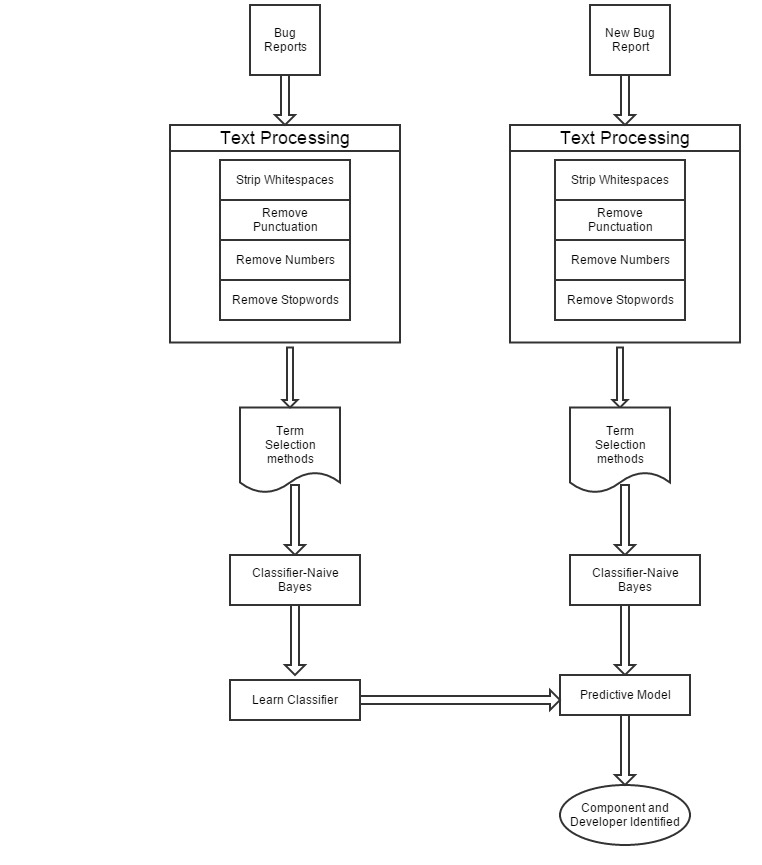
\includegraphics[height=15cm,width=15cm]{module}

\begin{figure}[hbt]
\begin{center}
\setboolean{@twoside}{false}

\includepdf[pages=12, offset =75 -75]{review3_v3.pdf}
\caption{MODULE DIAGRAM}
\end{center}
\end{figure}
%\section{Architecture Diagram}
%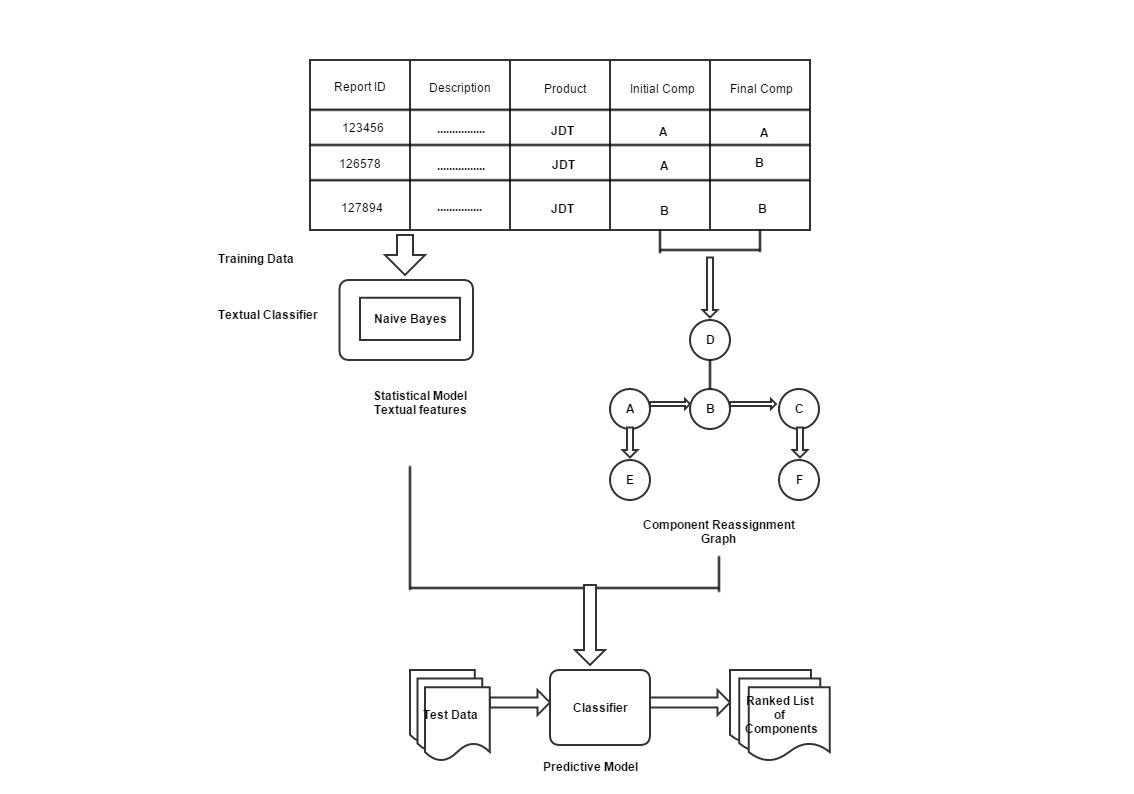
\includegraphics[height=15cm,width=17.5cm]{architecture}

%\setboolean{@twoside}{false}
%
\includepdf[left=1.5in,scale=0.8,pages=11]{review3_v3.pdf}

\newpage
\begin{figure}[hbt]
\begin{center}

\includepdf[pages=11, offset =75 -75]{review3_v3.pdf}
\caption{ARCHITECTURE DIAGRAM}
\end{center}

\end{figure}



%\section{Module Diagram}
%\begin{figure}[H]
%\input{module.pdf_tex}
%\end{figure}